\chapter{Introduction}
\thispagestyle{plain}

Scheduling is a decision-making process that plays an important role in most manufacturing and service industries. %\ref{}. 
Scheduling problems arise in almost any type of industrial production facilities where given tasks need to be processes using specified resources. In a chemical process, production must be planned such that equipment, material and utilities are available at the manufacturing facility when they are needed to realize the production tasks. Production scheduling comprises the activity of planning in detail the production of a product or products in a given production facility. It boils down to the following main decisions \citep{HARJUNKOSKI2014161}:
\begin{itemize}
\item What production tasks to execute?
\item Where to process the production tasks?
\item In which sequence to produce?
\item When to execute the production tasks?
\end{itemize}

For batch processes, short-term scheduling deals with the allocation of a set of limited resources over time to manufacture one or more products following a batch recipe \citep{MENDEZ}. Existing approaches rely on network-bsaed representation. Under the state-task network representation \citep{KONDILI1993211}, a task node is linked to a state node via an arc if the state is consumed or produced by the task. An example of a state task network is given in Fig. \ref{fig:STN}.

Alternatively, if units, states (materials) and utilities are viewed as resources consumed/produced by the task, then task-nodes are linked to resource-nodes, and the representation is referred to as a resource-task network (Fig. \ref{fig:RTN}). 

\begin{figure}[htb]
\centering
\fbox{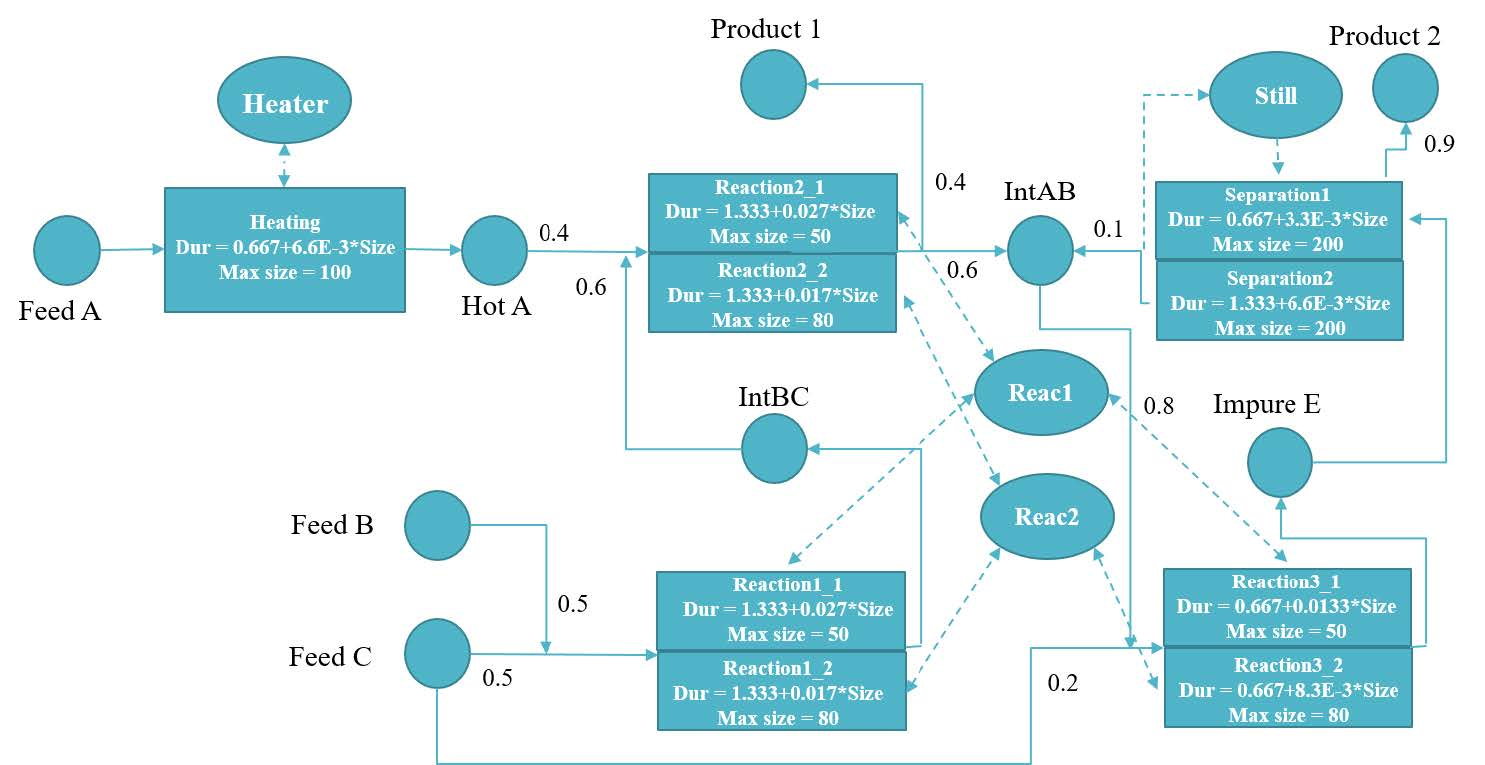
\includegraphics[width=\linewidth]{Images/RTN.jpg}}
\caption{Resource task network}
\label{fig:RTN}
\end{figure}

There has been significant development of optimization approaches to scheduling over the last two decades. Early attempts to establish general scheduling algorithms were based on the discretization of the time horizon into a number of intervals of equal and fixed duration. In such a model, all system events are forced to coincide with one of the interval boundaries. 
Such a mathematical programming approach for the scheduling of multi-purpose, multi-product batch plants was proposed by \cite{KONDILI1993211}. The main limitation of this approach resulted from the fact that the duration of all processing tasks must be a multiple of the discretization time, which implied a formulation with a high number of decision variables for reasonable accuracy for realistic applications.
\cite{SHAH1993229} developed specific solution techniques for the proposed formulation so as to reduce the computational time. However, the discretization problem was still present. This encouraged work towards the development of efficient methods based on continuous-time representations, which was first introduced for scheduling problems by \cite{SAHINIDIS199185}.

Subsequently, several continuous time models for the scheduling of batch plants were developed over the next two decades. Five of them are described in Chapter \ref{chap:models}:
\begin{enumerate}
\item \cite{Castro}
\item \cite{Maravelias}
\item \cite{Gimenez}
\item \cite{Ierapetritou}
\item \cite{Karimi}
\end{enumerate}

\label{uncertaintysection}
In realistic scenarios, many of the parameters associated with scheduling are not known exactly. Parameters such as processing time, yields, prices, etc. can vary with respect to time and are subject to unexpected deviations. Robust optimization is an approach that has been suggested to mitigate these uncertainties while designing a schedule. Robust optimization seeks to generate a solution that is immune to uncertainty by ensuring that it remains feasible for all possible realizations of the uncertain parameters from within a set chosen \emph{a priori} by the modeler.

This work supports two frameworks to handle uncertainty of parameters:

\begin{itemize}
\item \textbf{Static Robust Optimization: } The first application of robust optimization in process scheduling was by \cite{LIN20041069}. This work, which utilized box uncertainty sets, was later extended by \cite{JANAK2007171} to consider uncertainty sets derived from probabilistic information. \cite{LiIerapetritou} considered box, ellipsoidal and budget uncertainty sets. All these single-stage approaches are collectively referred to as Static Robust Optimization (SRO).

\item \textbf{Adjustable Robust Optimization: } SRO approaches are generally conservative, as they assume that all of the decisions have to be made 	``here-and-now'', before the schedule begins to be implemented. In reality, many of the decisions can be ``wait-and-see'', meaning that they can be delayed until a later point when the a subset of the uncertain parameters have revealed their values. To handle such multi-stage decision making strategies, Adjustable Robust Optimization (ARO) is used, where an optimal policy is derived instead of a single, static solution. The optimal policy constitutes a family of solutions that are parameterized in the uncertain parameter realizations \citep{lappas}.

\end{itemize}


This report describes the design and usage of an online webtool built to illustrate the procedure of building a scheduling instance and obtaining/interpreting results. The tool can be accessed online at \url{gounaris.cheme.cmu.edu/CMUPSO}. For instances involving uncertain parameters, \url{gounaris.cheme.cmu.edu/webtool6.0} should be used.